\subsection{Ejercicio 7}
\graphicspath{ {img/07} }

Thunderbird es un lector de correo con un gran número de funcionalidades adicionales, como calendarios, contactos y, más importante en nuestro caso, permite utilizar PGP para cifrar y firmar los correos.

Para añadir las claves se utiliza la herramienta \texttt{Gestor de claves PGP}, donde se pueden importar los pares de claves completos o solo las claves públicas, como se muestra a continuación:

\begin{figure}[H]
    \centering
    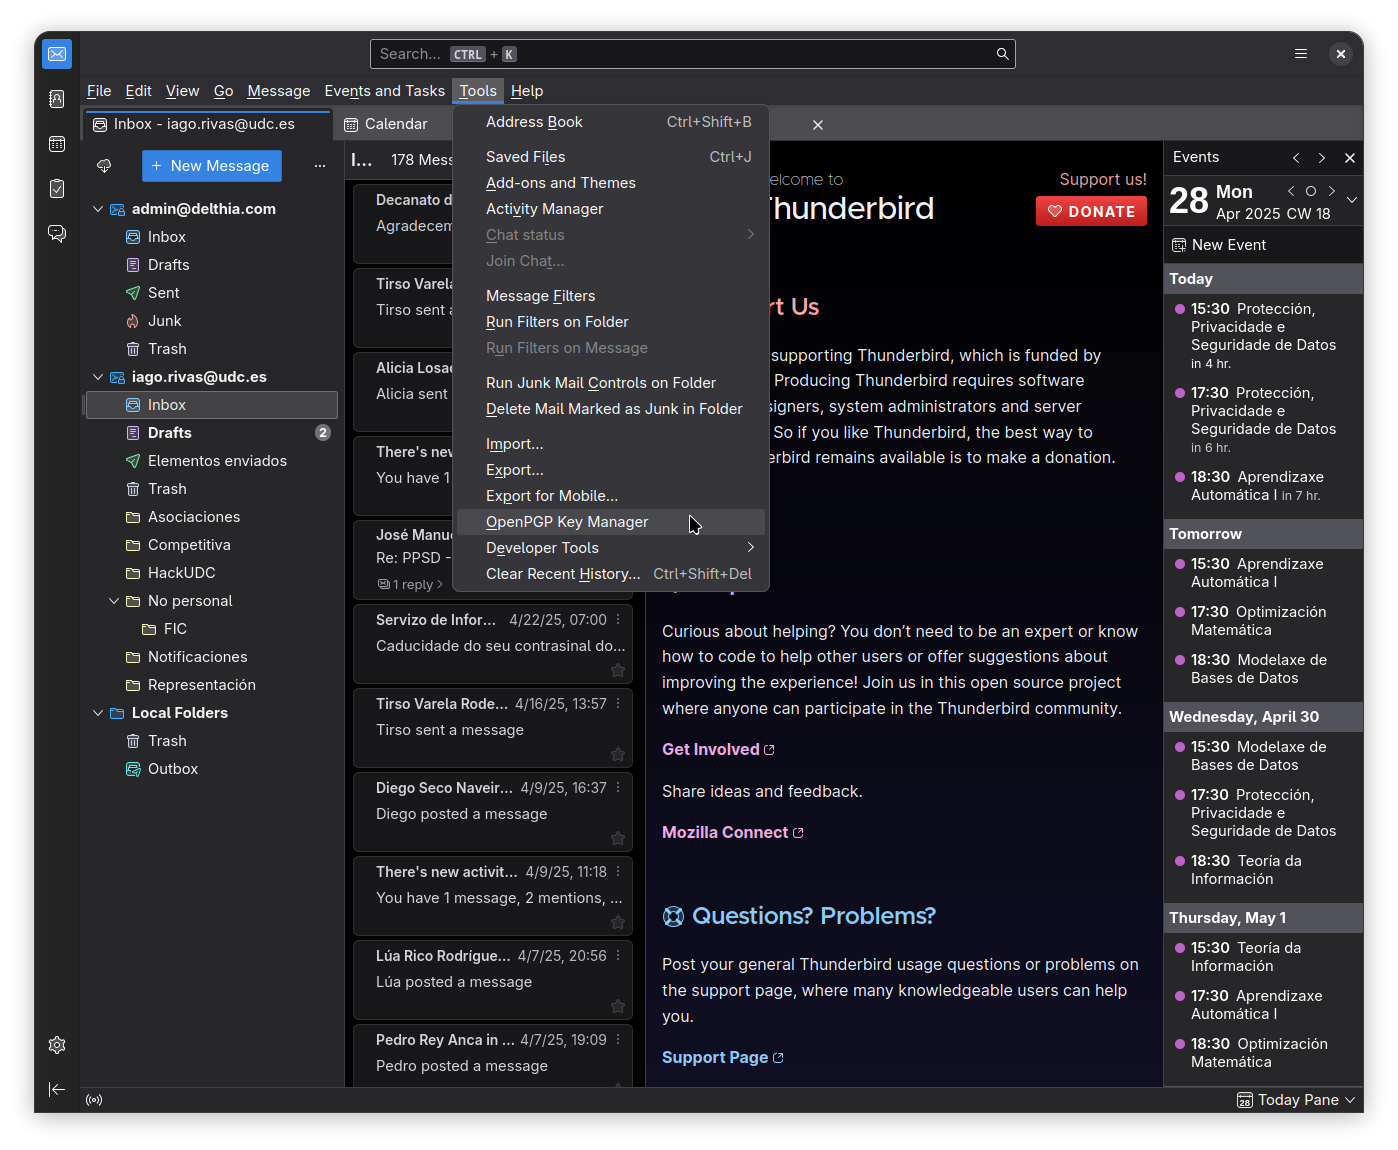
\includegraphics[width=\textwidth]{thunderbird-tools-menu.png}
    \caption{Menú con la herramienta “Gestión de claves OpenPGP”}
\end{figure}

\begin{figure}[H]
    \centering
    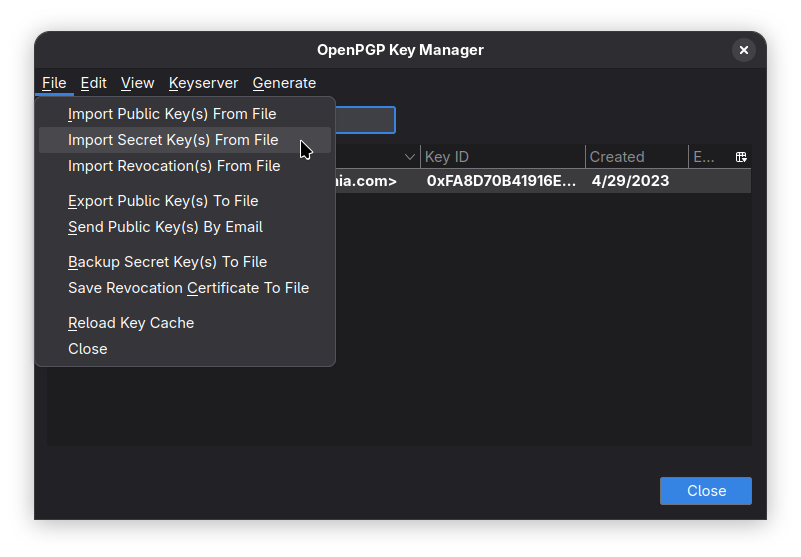
\includegraphics[width=10cm]{thunderbird-keymanager.png}
    \caption{Importación de claves en la herramienta “Gestión de claves OpenPGP”}
\end{figure}

\begin{figure}[H]
    \centering
    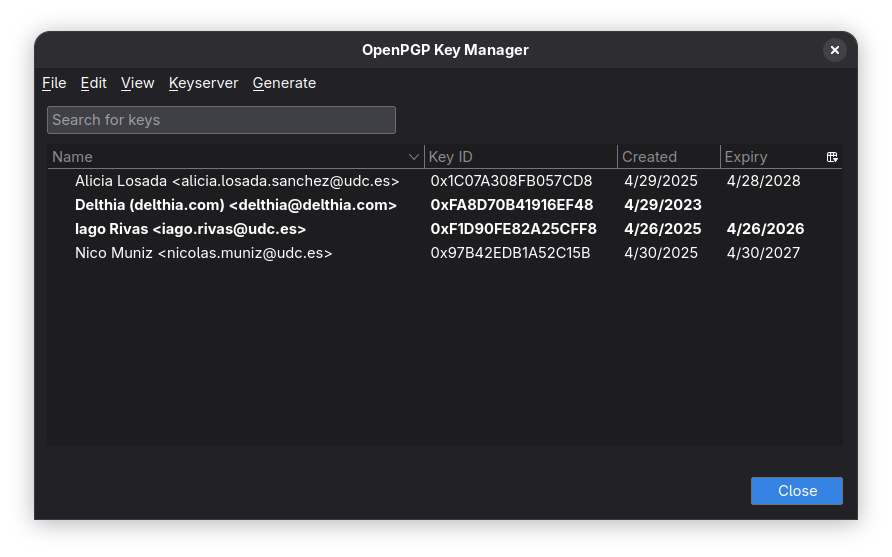
\includegraphics[width=10cm]{thunderbird-keymanager-keys.png}
    \caption{Claves PGP importadas en Thunderbird}
\end{figure}

Ahora, encriptar un correo es cuestión de selecciónar la opción “Encriptar” que se habilitará en la ventana de redacción, justo al lado del botón enviar. Junto a este botón hay un desplegable con tres opciones:
\begin{itemize}
    \item{\underline{Firmar:} Firma el correo con la clave del remitente. No afecta a la capacidad de leer el correo del destinatario.}
    \item{\underline{Encriptar:} Encripta el correo con la clave del destinatario, por lo que es necesario conocer la clave pública del mismo. Además, el destinatario no podrá leer el correo sin desencriptarlo con su clave privada. Existe una opción que permite encriptar también el asunto.}
    \item{\underline{Firmar y encriptar:} El corroe se firma y se cifra. Esto permite mantener la privacidad en la comunicación y que solo el destinatario, que puede leer el correo, pueda comprobar también que el remitente es quien dice ser.}
\end{itemize}

En estos casos el mensaje se envía como un bloque cifrado, y en caso de solo firmarse, se adjunta la firma. En otro lector de correo, por ejemplo la versión web de Outlook, no podremos leer el mensaje y tendremos que descargarlo para desencriptarlo con \texttt{gpg}, mientras que Thunderbird muestra automáticamente los mensajes cifrados como si no lo estuvieran, además de indicar claramente si tienen una firma y si es válida.

En primer lugar se envió un correo firmado, luego un correo cifrado y, por último, un correo cifrado y firmado.

\begin{figure}[H]
    \centering
    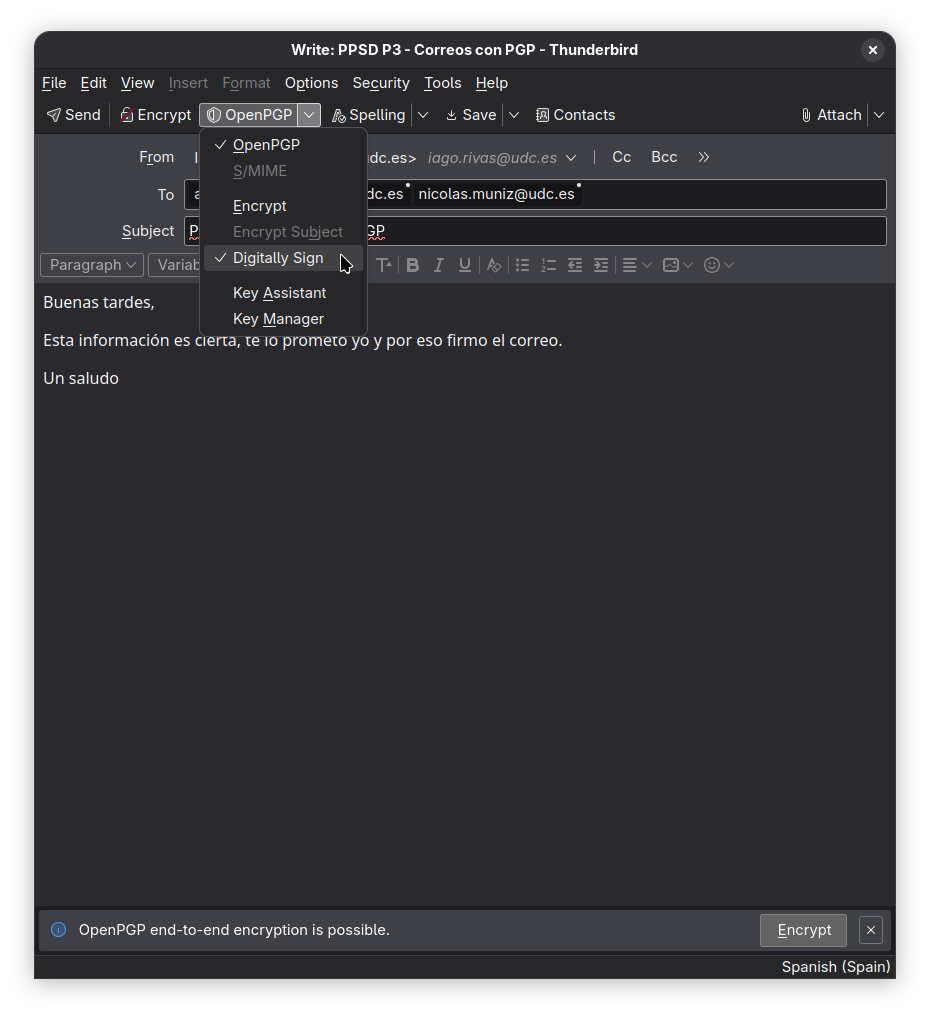
\includegraphics[width=10cm]{thunderbird-firmado.png}
    \caption{Envío de un correo firmado desde Thunderbird}
\end{figure}

\begin{figure}[H]
    \centering
    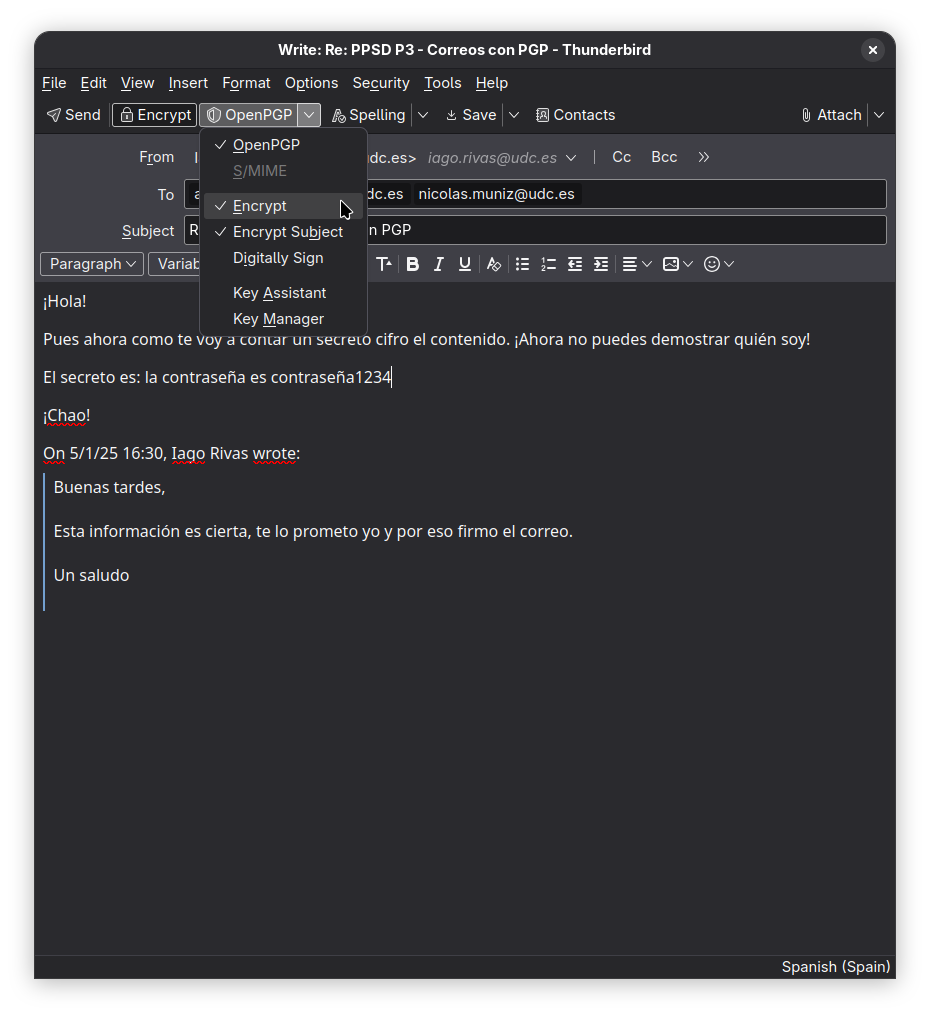
\includegraphics[width=10cm]{thunderbird-cifrado.png}
    \caption{Envío de un correo cifrado desde Thunderbird}
\end{figure}

\begin{figure}[H]
    \centering
    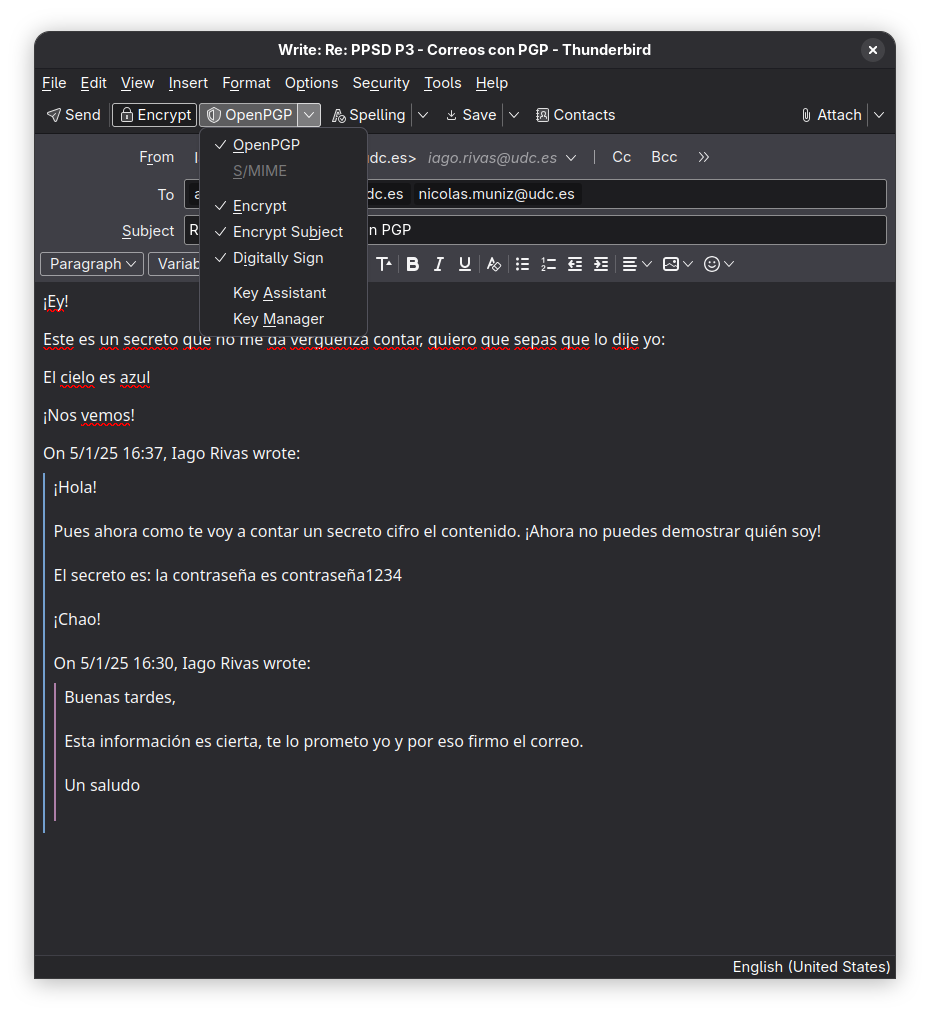
\includegraphics[width=10cm]{thunderbird-cifrado-firmado.png}
    \caption{Envío de un correo cifrado y firmado desde Thunderbird}
\end{figure}

El destinatario del correo podrá ver de forma clara que el correo estába cifrado y si tiene una firma válida, tal y como se muestra a continuación:

\begin{tcolorbox}[
    colback=orange!5!white,
    colframe=orange!75!black,
    title=El indicador de cifrado
]
Una vez configurado GPG en Thunderbird el funcionamiento es el de un cliente de correo habitual, con una opción de cifrado que, si se utiliza, automáticamente cifra el mensaje antes de enviarlo y lo muestra descifrado en el cliente. Además, mostrará un indicador cuando el mensaje está cifrado y/o firmado.

\begin{figure}[H]
    \centering
    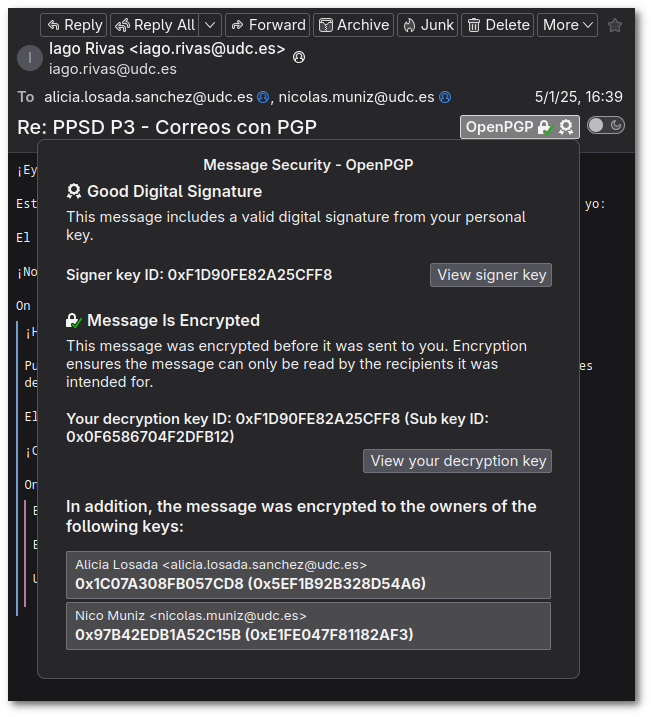
\includegraphics[width=8cm]{thunderbird-indicador-sombra.png}
    \caption{Indicador de cifrado en Thunderbird}
    \label{fig:indicador-cifrado}
\end{figure}

En caso de que se muestre un candado, sabremos que el mensaje está cifrado. Si aparece una insignia, el mensaje está firmado y, salvo que se muestre un error, la firma es válida.

Al hacer clic en el indicador vemos más detalles, tal y como se muestra en la figura \ref{fig:indicador-cifrado}.
\end{tcolorbox}

%\begin{figure}[H]
%    \centering
%    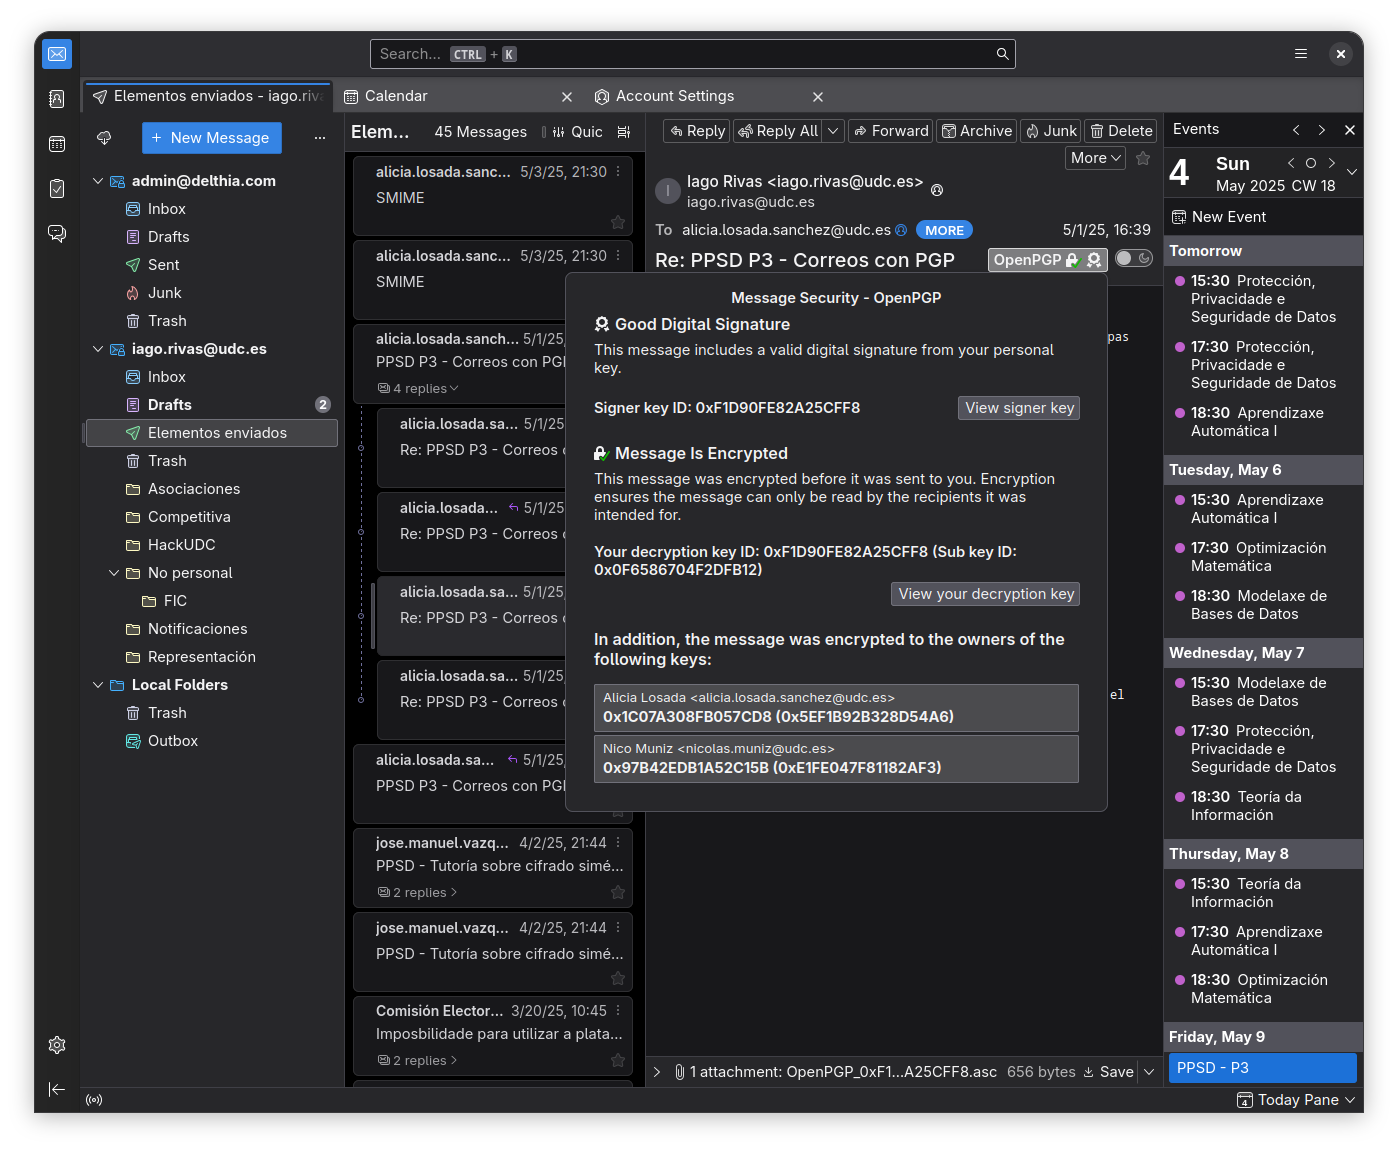
\includegraphics[width=10cm]{thunderbird-detalles.png}
%    \caption{Detalles del envío cifrado y firmado}
%\end{figure}
